% Author: Malte, DE7LMS
% Year: 2022
% E_TH209 Four Different Yagis

\usepackage{amsmath}
\usepackage{unicode-math}
\setmathfont{Fira Math}
\setmathfont[range=up]{Roboto}
\setmathfont[range=it]{Roboto-Italic}
\setmathfont[range=\int]{Fira Math}
\usepackage[euler]{textgreek}

\begin{document}

% horizontal
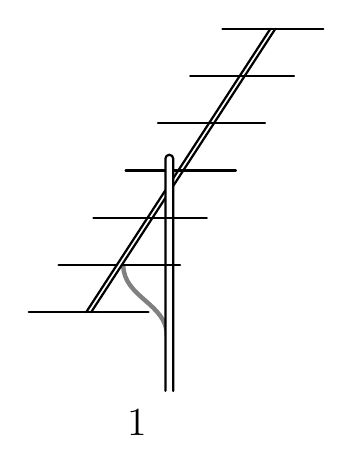
\begin{tikzpicture}[thick, x={(1cm,0)}, y={(2.6mm,4mm)}, z=({0,1cm}), line cap=round]
  % cable
  \path[gray, ultra thick, line cap=butt]
    (0.02,2.5*1.5,-1.8) edge[out=90,in=-90] (0.05,1.5,0);
  % boom
  \draw[xshift=-0.9pt] (0,0,0) -- (0,9,0);
  \draw[xshift=0.9pt] (0,0,0) -- (0,9,0);
  % directors
  \foreach \d/\y in {0.7/3,0.68/4,0.66/5,0.64/6} {
    \draw (-\d,\y*1.5,0) -- (\d,\y*1.5,0);
  }
  % pole
  \draw[rounded corners=.5mm, fill=white]
    (0,2.5*1.5,-2.5) -- ++(0,0,3) -- ++(.1,0,0) -- ++(0,0,-3)
    node[below=4mm,left=2mm,font=\Large] {1};
  % reflector
  \foreach \d/\y in {.76/0} {
    \draw (-\d,\y*1.5,0) -- (\d,\y*1.5,0);
  }
  % driven element
  \foreach \d/\y in {.74/1} {
    \draw[xshift=.9pt] (0,\y*1.5,0) -- (\d,\y*1.5,0);
    \draw[xshift=-.9pt] (0,\y*1.5,0) -- (-\d,\y*1.5,0);
  }
  % directors
  \foreach \d/\y in {0.72/2} {
    \draw (-\d,\y*1.5,0) -- (\d,\y*1.5,0);
  }
\end{tikzpicture}
\hskip-5mm
%vertical
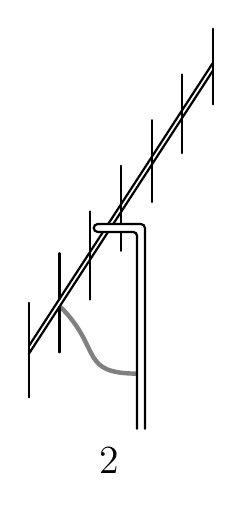
\begin{tikzpicture}[thick, x={(1cm,0)}, y={(2.6mm,4mm)}, z=({0,1cm}), line cap=round]
  % cable
  \path[gray, ultra thick, line cap=butt]
    (0.42,2.5*1.5,-1.8) edge[out=180,in=-45,looseness=1.5] (0.04,1.38,0);
  % boom
  \draw[yshift=-1.4pt] (0,0,0) -- (0,9,0);
  \draw[yshift=1.4pt] (0,0,0) -- (0,9,0);
  % directors
  \foreach \d/\y in {0.54/3,0.52/4,0.5/5,0.48/6} {
    \draw (0,\y*1.5,-\d) -- (0,\y*1.5,\d);
  }
  % pole
  \draw[rounded corners=.5mm,fill=white]
    (0.4,2.5*1.5,-2.5) -- ++(0,0,2.5) -- ++(-.55,0,0) -- ++(0,0,.1) -- ++(.65,0,0) -- ++(0,0,-2.6)
    node[below=4mm,left=2mm,font=\Large] {2};
  % directors
  \foreach \d/\y in {0.56/2} {
    \draw (0,\y*1.5,-\d) -- (0,\y*1.5,\d);
  }
  % driven element
  \foreach \d/\y in {.58/1} {
    \draw[yshift=1.4pt] (0,1.5,0) -- (0,1.5,\d);
    \draw[yshift=-1.4pt] (0,1.5,0) -- (0,1.5,-\d);
  }
  % reflector
  \foreach \d/\y in {.6/0} {
    \draw (0,0,-\d) -- (0,0,\d);
  }
\end{tikzpicture}
\hskip-5mm
%cross
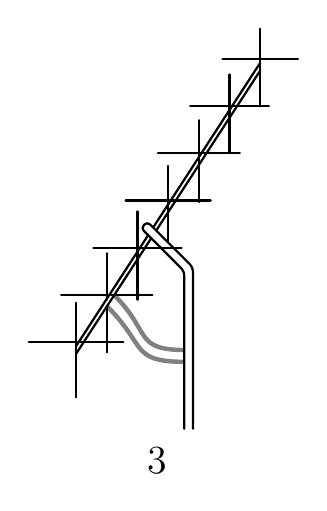
\begin{tikzpicture}[thick, x={(1cm,0)}, y={(2.6mm,4mm)}, z=({0,1cm}), line cap=round]
  % cables
  \path[gray, ultra thick, line cap=butt]
    (0.42,2.5*1.5,-1.65) edge[out=180,in=-45,looseness=1.5] (0.04,1.38,0);
  \path[gray, ultra thick, line cap=butt]
    (0.42,2.5*1.5,-1.5) edge[out=180,in=-45,looseness=1.5] (0.04,1.73,0);
  % boom
  \draw[yshift=-1.4pt] (0,0,0) -- (0,9,0);
  \draw[yshift=1.4pt] (0,0,0) -- (0,9,0);
  % directors
  \foreach \d/\y in {0.54/3,0.52/4,0.5/5,0.48/6} {
    \draw (0,\y*1.5,-\d) -- (0,\y*1.5,\d);
    \draw[yshift=2.8pt] (-\d,\y*1.5,0) -- (\d,\y*1.5,0);
  }
  % pole
  \draw[rounded corners=.5mm,fill=white]
    (0.4,2.5*1.5,-2.5) -- ++(0,0,2) -- ++(-.55,0,.55) -- ++(.08,0,.08) -- ++(.58,0,-.58) -- ++(0,0,-2.05)
    node[below=4mm,left=2mm,font=\Large] {3};
  \foreach \d/\y in {.58/1} {
    % vertical driven element
    \draw[yshift=1.4pt] (0,1.5,0) -- (0,1.5,\d);
    \draw[yshift=-1.4pt] (0,1.5,0) -- (0,1.5,-\d);
    % horizontal driven element
    \draw[yshift=2.8pt] (-\d,1.5,0) -- (\d,1.5,0);
  }
  % reflector
  \foreach \d/\y in {.6/0} {
    \draw (0,0,-\d) -- (0,0,\d);
    \draw[yshift=2.8pt] (-\d,0,0) -- (\d,0,0);
  }
  % directors
  \foreach \d/\y in {0.56/2} {
    \draw (0,\y*1.5,-\d) -- (0,\y*1.5,\d);
    \draw[yshift=2.8pt] (-\d,\y*1.5,0) -- (\d,\y*1.5,0);
  }
\end{tikzpicture}
\hskip-10mm
%circular
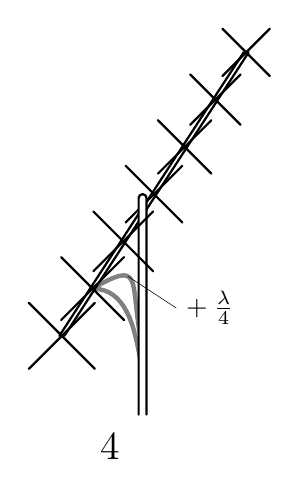
\begin{tikzpicture}[thick, x={(1cm,0)}, y={(2.6mm,4mm)}, z=({0,1cm}), line cap=round]
  % cable
  \path[gray, ultra thick, line cap=butt]
    (0.02,2.5*1.5,-1.8) edge[out=100,in=0] (0,1.5,0)
    (0.02,2.5*1.5,-1.5) edge[out=100,in=30,looseness=2.2] node[pos=0.6] (marker) {} (0,1.5,0);
  % boom
  \draw[xshift=-0.9pt] (0,0,0) -- (0,9,0);
  \draw[xshift=0.9pt] (0,0,0) -- (0,9,0);
  % directors
  \foreach \d/\y in {0.36/3,0.34/4,0.32/5,0.3/6} {
    \draw (-\d,\y*1.5,-\d) -- (\d,\y*1.5,\d);
    \draw (-\d,\y*1.5,\d) -- (\d,\y*1.5,-\d);
  }
  % pole
  \draw[rounded corners=.5mm, fill=white]
    (0,2.5*1.5,-2.5) -- ++(0,0,2.8) -- ++(.1,0,0) -- ++(0,0,-2.8)
    node[below=4mm,left=2mm,font=\Large] {4};
  % marker
  \node[xshift=10mm,yshift=-4mm, inner sep=1pt] at (marker) (marker text) {${}+\frac\lambda4$};
  \path[very thin]
    (marker.center) edge (marker text.west);
  % reflector, driven elements, directors
  \foreach \d/\y in {0.42/0,0.40/1,0.38/2} {
    \draw (-\d,\y*1.5,-\d) -- (\d,\y*1.5,\d);
    \draw (-\d,\y*1.5,\d) -- (\d,\y*1.5,-\d);
  }
\end{tikzpicture}

\end{document}
